\documentclass{standalone}

\usepackage[euler-digits]{eulervm}

\usepackage{tikz}
%\tikzset{every node/.style={draw=none,minimum size=2mm,inner sep=0pt}}
\tikzset{every node/.style={circle,draw,minimum size=6mm,inner sep=0pt}}

\begin{document}
    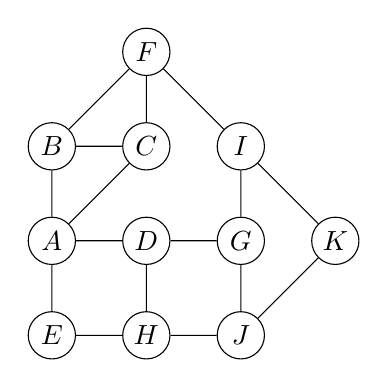
\begin{tikzpicture}[scale=1.2]
      \node (A) at (0,1) {$A$};
      \node (B) at (0,2) {$B$};
      \node (C) at (1,2) {$C$};
      \node (D) at (1,1) {$D$};
      \node (E) at (0,0) {$E$};
      \node (F) at (1,3) {$F$};
      \node (G) at (2,1) {$G$};
      \node (H) at (1,0) {$H$};
      \node (I) at (2,2) {$I$};
      \node (J) at (2,0) {$J$};
      \node (K) at (3,1) {$K$};

      \draw (D) -- (H) -- (E) -- (A) --(B) -- (F) -- (C) -- (A) -- (D) -- (G) -- (J) -- (H);
      \draw (J) -- (K) -- (I) -- (F);
      \draw (I) -- (G);
      \draw (B) -- (C);
    \end{tikzpicture}
\end{document}
